\documentclass[letterpaper]{article}
\usepackage[utf8]{inputenc}
\usepackage{authblk}
\usepackage{hyperref}
\usepackage{graphicx}
\usepackage{makecell}
\usepackage{draftwatermark}
\SetWatermarkText{DRAFT}
\SetWatermarkScale{4}

\usepackage[usenames,dvipsnames,svgnames,table]{xcolor}

\definecolor{teal}{HTML}{008080}

\hypersetup {
  colorlinks = true, linkcolor = teal, citecolor = teal, urlcolor = teal,
  pdfauthor = {Beauchesne, David},
}

\renewcommand\Affilfont{\itshape\small}
\setcounter{section}{0}

\begin{document}

\title{
  \uppercase {Thinking outside the box - predicting biotic interactions in data-poor environments}
}
\uppercase{

\author[1*]{\textit{David Beauchesne}}
\author[2]{\textit{Philippe Desjardins-Proulx}}
\author[3]{\textit{Philippe Archambault}}
\author[2]{\textit{Dominique Gravel}}
}
\affil[*]{email: \href{mailto:david.beauchesne@uqar.ca}{david.beauchesne@uqar.ca}}
\affil[1]{Universit\'e du Qu\'ebec à Rimouski}
\affil[2]{Universit\'e de Sherbrooke}
\affil[3]{Université Laval}
\date{\today}
\maketitle

%ADD RUNNING TITLE HERE, MUST NOT EXCEED 55 CHARACTERS AND SPACES

%UP TO 8 KEYWORDS
% \keywords{predicting biotic interactions, machine learning, food webs, estuary and gulf of St.Lawrence}

\newpage

% ---------------------------------
% ---------------------------------
%           ABSTRACT
% ---------------------------------
% ---------------------------------
\section{Abstract} % about 200 words
% \\TODO: verify 94 food webs

Large networks of ecological interactions, such as food webs, are complex to characterize, be it empirically or theoretically. The former requires exhaustive observations, while the latter generally requires ample data to be validated. We therefore wondered whether readily available data, namely empirically described interactions in a variety of ecosystems, could be combined to predict species interactions in data deficient ecosystems. To test this, we built a biotic interactions catalogue from a collection of \textit{94} empirical food webs, detailed predator-prey interaction databases and interactions from the Global Biotic Interactions (GloBI) database. We used an unsupervised machine learning method to predict interactions between any given set of taxa, given pairwise taxonomic proximity and known consumer and resource sets found in the interaction catalogue. Initial results suggest that pairwise interactions can be predicted with high accuracy. Although results are seemingly dependent on the comprehensiveness of the catalogue knowledge of taxonomy was found to complement well the catalogue and improve predictions, especially as empirical information available diminished. Given it’s high accuracy, this methodology could democratize the use of food webs and network level descriptors in remote location where empirical data is hard to gather. Network characteristics could then be efficiently evaluated and correlated to levels of environmental stressors in order to improve vulnerability assessments of ecosystems to global changes, opening promising avenues for further research and for management initiatives.

% ---------------------------------
% ---------------------------------
%           INTRODUCTION
% ---------------------------------
% ---------------------------------
\section{Introduction}
Large networks of ecological interactions, such as food webs, are complex to characterize (Martinez, 1992; Pascual and Dunne, 2006). Empirical descriptions require exhaustive observations, while theoretical inference generally requires ample data to be validated. For this reason, studies focusing on communities of interacting species remain understudied, even though we acknowledge the importance of considering the reticulated nature of complex networks (Ings et al. 2007; Tylianakis et al. 2008). When time is of the essence, the long term studies required quickly become impractical and the use of network level approaches is relegated to the sideline.

Alternatively, a currently evolving approach is to predict interactions using proxies such as functional traits, phylogenies and spatial distributions (e.g. Gravel et al., 2013; Morales-Castilla et al., 2015; Bartomeus et al. 2016). For example, multiple traits can play a significant role in community dynamics and influence the presence and intensity of biotic interactions, like the influence of body size on predator-prey interactions, a literal take on \textit{big fish eats small fish} (Cohen et al., 2003; Brose et al., 2006; Gravel et al. 2013). However, the time required to gather the necessary data to apply those methods may still be restrictive, or the data be unavailable altogether, so much so that other methods have been developed to fill the gaps in knowledge (e.g. Schrodt et al. 2016).

We therefore wondered whether more readily available data could be used to infer interactions in data deficient ecosystems. There is an increasing amount of data describing worldwide species interactions, some freely available through the Global Biotic Interactions (GloBI) database (Poelen et al. 2014). Another readily available piece of information on species is their taxonomy, through initiatives like the World Register of Marine Species (WoRMS; Bailly et al. 2016). More than simple nomenclature, evolutionary processes are thought to influence consumer-resource relationships (Mouquet et al. 2012; Rohr and Bsacompte, 2014) so that taxonomically related species would be more likely to share similar types of both consumers and resources (Eklof et al. 2012; Morales-Castilla et al. 2015; Gray et al. 2015). Based on that assumption, taxonomy might be useful in predicting interactions for species lacking detailed information on their biology, but which have a taxonomically related species for which such information is available. The objective of this work is thus to combine empirical biotic interactions originating from a variety of ecosystems with taxonomic relatedness to predict interactions in data deficient ecosystems. As an example, we compare the observed interactions in the Southern Gulf of St Lawrence (Savenkoff et al. 2004) with predictions made using our approach.

% ---------------------------------
% ---------------------------------
%             METHODS
% ---------------------------------
% ---------------------------------
\section{Methods}
The objective of our methodology is to predict the interactions between all pairs of taxa within an arbitrary set $N_1$, using a set of taxa $N_0$ with empirically described interactions from which we can extract pairs of consumers and resources and their taxonomy. We couple the use of empirical data with an unsupervised machine learning method to achieve this.

 \subsection{Biotic interaction catalogue}
   % \\TODO: Add reference GlobalWeb database (http://globalwebdb.com)
   % \\TODO: Verify references to add

We built a biotic interaction catalogue to serve as a set of taxa $N_0$ for training the algorithm with empirically described interactions. The empirical data used to construct the interaction catalogue was gathered in two successive steps. The first consisted of gathering data from a collection of 94 empirical food webs in marine and coastal ecosystems from which we extracted pairwise taxa interactions (Brose et al. 2005; Kortsch et al. 2015; GlobalWeb database). We also used a detailed predator-prey interaction database describing trophic relationships between \textit{XX} predators and their prey (Barnes et al. 2008). From these datasets, only interactions between taxa at the taxonomic scale of the family or higher were selected for inclusion in the catalogue.

As empirical food webs are vastly dominated by non-interactions, these datasets yielded a highly skewed distribution of interactions vs non-interactions. To counterbalance this, the second step of data compilation consisted of extracting observed interactions from the Global Biotic Interaction (GloBI) database (ref), which describes binary interactions for a wide range of taxa worldwide. We extracted all interactions available on GloBI for species belonging to the families of taxa identified through step 1. Interactions were extracted using the rGloBI package in R (ref). As for step 1, only interactions between taxa at the taxonomic scale of the family or higher were retained

The nomenclature used between datasets and food webs varied substantially. Taxa names thus had to be verified, modified according to the scientific nomenclature and validated. This process was performed using the Taxize package in R (ref) and manually verified for errors. The same package was used to extract the taxonomy of all taxa for which interactions were obtained in previous steps. The complete R code and data used for the catalogue is available at \href{https://github.com/david-beauchesne/Interaction_catalog}{https://github.com/david-beauchesne/Interaction\_catalog}.

  \subsection{Unsupervised machine learning}
We use the \textit{K}-nearest neighbor (KNN) algorithm (\textbf{ref}) to predict pairwise interactions for a set of taxa \textit{S}. The KNN algorithm predicts missing entries or proposes additional entries by a majority vote based on the \textit{K} nearest (\textit{i.e.} most similar) entries (see Box 1 for an example). In this case, taxa are described by a set of resources when considered as a consumer, a set of consumers when considered as a resource and their taxonomy (\textit{i.e.} kingdom, phylum, class, order, family, genus, species). Similarity between taxa was evaluated using the Tanimoto similarity measure (\textbf{ref}), which compares two vectors with \textit{i} elements based on the number of elements they share and contain:

\begin{equation}
  tanimoto(\mathbf{x}, \mathbf{y}) = \frac{\sum_i x_i \land y_i}{\sum_i x_i \lor y_i},
\end{equation}

where $\land$ is bitwise \emph{and}, while $\lor$ is the bitwise \emph{or} operators. Adding a weighing scheme, we can measure the similarity using two different sets of vectors with \textit{i} and \textit{j} elements, respectively.

\begin{equation}
  tanimoto_t(\mathbf{x}, \mathbf{y}, w_t) = w_ttanimoto(\mathbf{x_i}, \mathbf{y_i}) + (1 - w_t)tanimoto(\mathbf{x_j}, \mathbf{y_j}),
\end{equation}

where $w_t$ is the weight given to vector \textit{i}, $\mathbf{x_i}$, $\mathbf{y_i}$ are the resource or consumer sets of the two taxa and $\mathbf{x_j}$ and $\mathbf{y_j}$ are the vectors for the taxonomy of two taxa. When $w_t$ = 0 only resource or consumer sets are used to compute similarity, while $w_t$ = 1 solely uses taxonomy.

  \subsection{Predicting interactions, Biotic predictor algorithm, Two-way Tanimoto algorithm, Feng shui name algorithm, Find a name for the algorithm}
% DG: iTunes is using this type of algorithm to recommend music, so that following its logic, I popose 'iEat'
% PA: ok voici des exemple: praedictio (prediction en latin); Taxoweb; praedictio commercium (prediction des interaction en latin); prediweb; bionet; Predictaxo; Nataxo


The XXX algorithm is built on a series of logical steps that ultimately predicts a candidate resources list $C_R$ for each taxon in $N_1$ (Figure \ref{fig:decision_diag}). For all consumer taxa $T_C$ in $N_1$, the algorithm first verify whether it has empirical resources $T_R$ listed in the catalogue (Step S1, Figure \ref{fig:decision_diag}). When it does, if $T_R$ are also in $N_1$, they are added as predicted resources for $T_C$ (S2, S3). This corresponds to what we refer to as the catalogue contribution to resource predictions. Two taxa in $N_1$ that are known to interact through the catalogue are automatically assumed to interact in $N_1$.

Otherwise, the algorithm passes to what we refer to as the predictive contribution to resource predictions (S4 to S16), with candidate resources for $T_C$ identified with the KNN algorithm. If $T_R$ are absent from $N_1$, K most similar resource $T_{R'}$ are identified in $N_1$ to add to $C_R$ (S4 to S7). Then for all $T_C$ in $N_1$, the algorithm identifies K most similar consumer $T_{C'}$ in $N_0$ and extracts their resource sets (S8). As before, if those resources are found in $N_1$ (S9) they are added to $C_R$ (S10 to S12), otherwise K most similar resources $T_{R'}$ are identified in $N_1$ (S13) to add to $C_R$ (S14 to S16). A simple working example is presented at Box 1. Note that other parameters are used in the algorithm, but not presented here for the sake of message clarity. A more comprehensive mathematical description of the algorithm and the parameters used is however available through Figure \ref{fig:decision_diag} and the complete R code and data used for the algorithm is available at \href{https://github.com/david-beauchesne/Predict_interactions}{https://github.com/david-beauchesne/Predict\_interactions}.


\subsection{Algorithm prediction accuracy}
We used the most extensive and taxonomically detailed datasets included in the catalogue (\textbf{ref}) to assess the prediction accuracy of the algorithm. Testing accuracy of a particular dataset was done by first removing from the catalogue all pairwise interacting taxa originating from that dataset. Accuracy was evaluated using three different statistics:

\begin{enumerate}
 \item $Score_y$ is the fraction of interactions correctly predicted:
     \begin{equation}
         Score_y = \frac{a}{a + c}
     \end{equation}

 \item $Score_{\neg y}$ is the fraction of non-interactions correctly predicted:
     \begin{equation}
       Score_{\neg y}  = \frac{d}{b + d}
     \end{equation}

 \item TSS, The True Skilled Statistics (TSS) evaluated prediction success by considering both true and false predictions, returning a value ranging from 1 (prefect predictions) to -1 (inverted predictions; \textbf{ref}): %Allouche, Tsoar et Kadmon 2006; Gravel et al. 2013
     \begin{equation}
       TSS = \frac{(ad - bc)}{(a + c)(b + d)}
     \end{equation}
\end{enumerate}

where $a$ is the number of links predicted and observed, $b$ is the number predicted but not observed, $c$ is the number of non-interaction predicted but interactions observed and $d$ is the number of non-interaction predicted absent and observed. These three statistics give a different perspective on prediction accuracy, focusing in turn on true interactions and non-interactions, and on both true and false predictions.

We evaluated the three statistics for the complete algorithm and for the catalogue and the predictions individually to evaluate their respective contribution to the algorithm predictive accuracy. Multiple $w_t$ values were also tested to evaluate whether taxa similarity measured as a function of resource/consumer sets or taxonomy contributed more significantly towards increased predictive accuracy. The same was done with multiple $K$ values.

Finally, we evaluated the influence of the comprehensiveness of the catalogue on prediction accuracy. We selected the arctic food web from Kortsch et al. (2015) as a test. This food web was selected as it is highly detailed taxonomically and because empirical data remains available for most of its taxa after its exclusion from the catalogue.
%DG: I don't get the previous sentence
We iteratively and randomly ($n$ = 50 randomizations) removed a percentage of empirical data describing the food web taxa from the catalogue before generating new predictions with the algorithm. We also tested $w_t$ values of 0.5 and 1 to evaluate whether taxonomic similarity could support predictive accuracy in cases when empirical data for species in $N_1$ in the catalogue is unavailable.

% ---------------------------------
% ---------------------------------
%            RESULTS
% ---------------------------------
% ---------------------------------
% \\TODO: Not MW, MT and accuracy score. The goal of the paper is to present the methodology and it just takes away from my main message. Accuracy score is taken out mainly because as non-interations vastly outnumber interactions, that graph essentially gives the same information as the score -y one. So now we would have three statistics instead of 4. Makes more sense I believe.
% \\TODO: include name of datasets used in figure captions

\section{Results}
    \subsection{Biotic interaction catalogue}
The data compilation process allowed us to build an interaction catalogue composed of 276708 pairwise interactions (interactions = 72110; non-interactions = 204598). A total of 9712 taxa (Superfamily = 15; Family = 591; Subfamily = 29; Tribe = 8; Genus = 1972; Species = 7097) are included in the catalogue, 4159 of which have data as consumers and 4375 as resources.

    \subsection{Algorithm predictive accuracy}
The overall predictive accuracy of the algorithm ranges between 80\% to almost 100\% in certain cases (Figure \ref{fig:multi_param}), except for one food web (\textit{i.e.} \textbf{ref}). Both interactions and non-interactions are well predicted by the algorithm. TSS scores are lower than $Score_y$ and $Score_{\neg y}$ due to misclassified interactions and non-interactions. This can also be observed through the effect of varying $K$ values, which increases the number of potential candidate resources for each taxa in the predictive portion of the algorithm. Prediction accuracy increases for interactions, while it decreases for non-interactions, as $K$ values increase.

Similarity being predominantly measured with resource/consumer sets ($w_t$ closer to 0) yielded better predictions than when measured with taxonomy ($w_t$ closer to 1; Figure \ref{fig:multi_param}). Resource/consumer sets therefore appears to serve as a better predictor of similarity between taxa for interactions predictions. It is nonetheless interesting to note that although the predictive contribution of the algorithm decreases as $w_t$ increases, an increased mean and decreased variability values for the TSS and $Score_y$ statistics is also observed (Figure \ref{fig:multi_param})). This suggests that while using taxonomy for similarity measurements yields lower predictive accuracy, it may also complement the catalogue contribution by predicting interactions not captured through empirical data, effectively increasing the predictive accuracy of the complete algorithm.

The partitioning of the catalogue and predictive portions of the algorithm shows that it is dependent on the comprehensiveness of the catalogue for high prediction accuracy (Figures \ref{fig:multi_param}, \ref{fig:catalog_pred}). As the amount of empirical data available in the catalogue decreases so does the overall accuracy of the algorithm (Figures \ref{fig:catalog_pred}). The predictive contribution of the algorithm however slows down the decrease in the prediction efficiency of the algorithm. Prediction accuracy still remains around 75\% with only 40\% of $N_1$ taxa found in the catalogue (Figures \ref{fig:catalog_pred}). Furthermore, the use of taxonomy for similarity measurements is more efficient as empirical data becomes scarcer and no different than resource/consumer sets for the complete algorithm when ample data is available (Figures \ref{fig:catalog_pred}).

    \subsection{Southern Gulf of Saint Lawrence}
As an example, we used the XXX algorithm to predict interactions in the Southern Gulf of Saint Lawrence (SGSL) in eastern Canada. The empirical data and taxa list come from Savenkoff et al. (2004). They present a list of 29 functional groups for a total of 80 taxa presented at least at taxonomical scale of the family. Other coarser taxa families were not used for this example (see Table S1 in Supplementary information (SI) and Savenkoff et al. 2004 for a complete description of functional groups). As their analysis was performed on the functional groups rather than the taxa themselves, we used the algorithm to predict interactions between all 80 taxa selected. We then aggregated them back to their original functional groups to compare with interactions presented in Savenkoff et al. (2004). In total, there were empirical data available in the catalogue for 78\% of SGSL taxa (62/80). The algorithm correctly predicted close to 80\% of interactions ($a$ = 135/170) and non-interactions ($d$ = 354/455) extracted from Savenkoff et al. (2004). It also predicted an additional 101 interactions ($c$) that were not noted in Savenkoff et al. (2004) and failed to predict 36 observed interactions that were ($c$), resulting in a TSS score of 0.57. A visual comparison of results obtained from the algorithm with interactions noted in Savenkoff et al. (2004) is available at Figure \ref{fig:SGSL}. The network presented is centered on the observed and predicted interactions of the capelin (\textit{Mallotus villosus}) and piscivorous small pelagic feeders (\textit{e.g. Scomber scombrus} and \textit{Illex illecebrosus}).

% SGSL accuracy results
% a           b             c           d           TSS         ScoreY1     ScoreY0         FSS
% 135.0000000 101.0000000  35.0000000 354.0000000   0.5721396   0.7941176   0.7780220   0.7824000

% ---------------------------------
% ---------------------------------
%           DISCUSSION
% ---------------------------------
% ---------------------------------
\section{Discussion}
\subsection{Algorithm accuracy}
We show that out of the box interaction inference for a set of taxa with incomplete or unavailable preexisting information can be achieved with high accuracy using a combination of empirical data describing biotic interactions and taxonomic relatedness. Although the efficiency of the algorithm is dependent on the comprehensiveness of the interactions catalogue, taxonomic proximity acts as a complement to increase the number of observed interactions correctly predicted. Taxonomic proximity also supports the efficiency of the algorithm when catalogue comprehensiveness decreases. Overall, we believe that the methods performs well and offers promising avenues for further research and management initiatives.

\subsection{Usefulness of taxonomic relatedness}
 While we found that taxonomy could be useful as a complement to predictions made using empirical data, the accuracy of predictions made using the KNN algorithm could be better. Other uses of this machine learning approach have been known to achieve much higher prediction rates (\textit{e.g.} \textbf{refs}), which suggests that taxonomy may not be the optimal proxy for predicting interactions. While evolutionary history plays a significant role in influencing consumer-resource trait matching and food web structure (\textbf{ref}), phylogenetic constraints do not account efficiently for certain traits such as body size (Eklöf and Stouffer 2015). Including traits like body size and metabolism as an additional component of this algorithm could thus help increasing overall prediction accuracy, especially in cases where the catalogue lacks data on taxa for which interactions have to be predicted. Although promising, such an approach would undermine the premise under which this method was built and which constitutes its main strength, $i.e.$ predicting interactions in data deficient environments using readily available data.
 %PA: Annie Scientific report pour body size

\subsection{Interactions classification}
That $Score_{y}$ and $Score_{\neg y}$ are inversely proportional2 means that non-interactions are misclassified as interactions in the process of increasing $Score_y$, consequently decreasing $Score_{\neg y}$. This could either stem from the algorithm poorly predicting non-interactions or from the empirical data itself. Accuracy evaluation assumes that non-interactions from empirical food web are observed data, yet it is usually not the case. Most empirical webs have a strong focus attributed to higher order consumer species and very little attention given to other taxa (\textbf{ref}). Furthermore, the methodologies used to obtain consumer-resource data usually relies on gut content analyses, which is efficient at observing interactions, but not so for absence of interactions (\textbf{ref}). Misclassified interactions could thus be real, albeit unobserved through empirical data available.

The St Lawrence example (Figure \ref{fig:SGSL} and SI) provides great material to discuss predictions in greater detail. The algorithm fails to predict 20\% of interactions presented in Savenkoff et al. (2004). Interactions that failed to be predicted were mainly centered on invertebrate species ($e.g.$ polychaetes and mollusks) and large functional groups described by coarse taxonomic categories ($e.g.$ diatoms) alongside few species in Savenkoff et al (2004) ($e.g.$ piscivorous small pelagic feeders; Table S3). As we focused on the taxa at least at the scale of family, it is likely that their functional groups had a broader range of possible interactions included than what the algorithm could predict using only a few taxa. Furthermore, the efficiency of the algorithm greatly depends on the underlying empirical data that defines the catalogue. If the empirical data used to build the catalogue focuses on higher order consumers, it should come as no surprise that the algorithm would be afflicted by the same limitations.

The algorithm also predicts substantially more interactions than those presented in Savenkoff et al. (2004) (Figure \ref{fig:SGSL}; Table S2). The catalogue is not currently built to take into account life stages of species. Considering life stages and the fact that they are not explicitely considered in the catalogue could explain additional interactions that seem suspicious at first, like the surprise amount of additional interactions predicted for small piscivorous pelagic feeders as consumers (Figure \ref{fig:SGSL}).

\subsection{Perspectives}

Probability, intensity of interactions (can influence greatly the interactions observed in nature) should be discussed as

Species spatial distributions.


Given the efficiency and simplicity of the XXX algorithm,

The simplicity of the XXX algorithm could prove useful for a variety of reasons



Given it’s high accuracy, this methodology could democratize the use of food webs and network level descriptors in remote location where empirical data is hard to gather. Network characteristics could then be efficiently evaluated and correlated to levels of environmental stressors in order to improve vulnerability assessments of ecosystems to global changes, opening promising avenues for further research and for management initiatives.



Democratizing the use of network level predictors
Management
Applied research in theoretical ecology
Adding interaction strength to predictions





\section{Acknowledgements}
We thank the Fond de Recherche Québécois Nature et Technologie (FRQNT) and the Natural Science and Engineering Council of Canada (CRSNG) for financial support. This project is also supported by Québec Océan, the Quebec Centre for Biodiversity Science (QCBS), and the Notre Golfe and CHONeII networks. We also wish to thank K. Cazelles for the help, constructive comments and suggestions.

\newpage
\subsection{Box 1}
The XXX algorithm follows a series of logical steps to predict resources for all taxa in an arbitrary set of taxa $N_1$ using a set of taxa $N_0$ with empirically described interactions from which we can extract sets of consumers and resources and their taxonomy. In this example, we are predicting interactions for a fictitious $N_1$
 = $\{T_1, T_9, T_{10},T_{11}, T_{12}\}$ using $N_0$ with information on 12 taxa. This catalogue holds information on consumer or resource for 10 taxa and the taxonomy for all 12 taxa in the list.

    \begin{table}[h!]
      \centering
      \begin{tabular}{cccc}
        \hline
        $N_0$ taxa ID & taxonomy &          resource &             consumer        \\
        \hline
        \hline
        $T_1$ &         $\{a, b, c\}$ &     $\{T_2, T_3, T_{12}\}$ &    $\{T_4\}$         \\
        $T_2$ &         $\{e, f, g\}$ &      &                          $\{T_1, T_5\}$    \\
        $T_3$ &         $\{i, j, k\}$ &      &                          $\{T_5\}$         \\
        $T_4$ &         $\{m, n, o\}$ &     $\{T_1, T_5\}$ &                              \\
        $T_5$ &         $\{a, b, d\}$ &     $\{T_8, T_9\}$ &            $\{T_4\}$         \\
        $T_6$ &         $\{i, q, r\}$ &     $\{T_2, T_8\}$ &            $\{T_4\}$         \\
        $T_7$ &         $\{e, f, h\}$ &      &                          $\{T_1, T_6\}$    \\
        $T_8$ &         $\{s, t, u\}$ &      &                          $\{T_5, T_6\}$    \\
        $T_9$ &         $\{s, t, v\}$ &      &                          $\{T_5\}$         \\
        $T_{10}$ &      $\{i, j, l\}$ &      &                                            \\
        $T_{11}$ &      $\{m, n, p\}$ &      &                                            \\
        $T_{12}$ &      $\{q, r, s\}$ &      &                          $\{T_1\}$         \\
        \hline
      \end{tabular}
    \end{table}

Similarity between all pairs of taxa in $N_0$ is measured for consumer, resource and taxonomic proximity using equation 1. The upper triangular matrix represents similarity measured with taxa sets of resources/consumers, while the lower triangular represents taxonomic similarities. For consumer/resource set similarities, values of 0 mean that similarity equals 0 for both similarity measurements.
\bigskip

    \centerline{$tanimoto(T_Cx, T_Cy)$ / $tanimoto(T_Rx, T_Ry)$ }

    \begin{table}[h!]
      \centering
      \small
      \begin{tabular}{c|ccccccccccccc}
        & $T_1$ & $T_2$ & $T_3$ & $T_4$ & $T_5$ & $T_6$ & $T_7$ & $T_8$ & $T_9$ & $T_{10}$ & $T_{11}$ & $T_{12}$ \\
        \hline
        $T_1$       & -     & 0     & 0         & 0     & 0/1   & 0.3/1     & 0         & 0         & 0         & 0     & 0     & 0         \\
        $T_2$       & 0     & -     & 0/0.5     & 0     & 0     & 0         & 0/0.3     & 0/0.3     & 0/0.5     & 0     & 0     & 0/0.5     \\
        $T_3$       & 0     & 0     & -         & 0     & 0     & 0         & 0         & 0/0.5     & 0/1       & 0     & 0     & 0         \\
        $T_4$       & 0     & 0     & 0         & -     & 0     & 0         & 0         & 0         & 0         & 0     & 0     & 0         \\
        $T_5$       & 0.5   & 0     & 0         & 0     & -     & 0.3/1     & 0         & 0         & 0         & 0     & 0     & 0         \\
        $T_6$       & 0     & 0     & 0.2       & 0     & 0     & -         & 0         & 0         & 0         & 0     & 0     & 0         \\
        $T_7$       & 0     & 0.5   & 0         & 0     & 0     & 0         & -         & 0/0.3     & 0         & 0     & 0     & 0/0.5     \\
        $T_8$       & 0     & 0     & 0         & 0     & 0     & 0         & 0         & -         & 0         & 0     & 0     & 0         \\
        $T_9$       & 0     & 0     & 0         & 0     & 0     & 0         & 0         & 0.5       & -         & 0     & 0     & 0         \\
        $T_{10}$    & 0     & 0     & 0.5       & 0     & 0     & 0.2       & 0         & 0         & 0         & -     & 0     & 0         \\
        $T_{11}$    & 0     & 0     & 0         & 0.5   & 0     & 0         & 0         & 0         & 0         & 0     & -     & 0         \\
        $T_{12}$    & 0     & 0     & 0         & 0     & 0     & 0.5       & 0         & 0.2       & 0.2       & 0     & 0     & -         \\
      \end{tabular}
    \end{table}

    \centerline{$tanimoto(T_Tx, T_Ty)$}
\bigskip

From these, the algorithm goes through logical steps (Figure \ref{fig:decision_diag}) to identify a candidate resource list $C_R$ for each taxon in $N_1$ using either empirical data directly or $K$ most similar taxa with equation 2. Going through the process for $T_1$, using $K$ = 1 and $w_t$ = 1:
\bigskip

\begin{table}[h!]
  \centering
  \small
  \begin{tabular}{cl}
      Steps \\
      \hline
      1        &$I(T_1,T_R)$ in $N_0$? \\
      2        &$T_R$ in $N_1$? \\
      4-7      &$T_2$ = no $\rightarrow$ $t(T_2, T_{R'}, w_t)$ = NA   \\
      4-7      &$T_3$ = no $\rightarrow$ $t(T_2, T_{R'}, w_t)$ = $T_{10}$ = 0.5 \\
      3        &$T_{12}$ = yes    \\  \\
      8        &$t(T_1, T_{C'}, w_t)$ = $T_5$ = 0.5            \\
      9        &I($T_5$,$T_R$) in $N_1$? \\
      13-16    &$T_8$ = no $\rightarrow$ $t(T_8, T_{R'}, w_t)$ = $T_9$ = 0.5  \\
      10-12    &$T_9$ = yes   \\
  \end{tabular}
  \begin{tabular}{c|c}
     & \\  \\  \\  \\  \\  \\  \\  \\  \\  \\  \\
  \end{tabular}
  \begin{tabular}{cc}
      Catalogue   & Prediction \\
      \hline \\ \\
      $\{\}$    & $\{\}$            \\
      $\{\}$    & $\{T_{10}\}$      \\
      $\{T_{12}\}$    & $\{T_{10}\}$      \\  \\  \\ \\
      $\{T_{12}\}$    & $\{T_9, T_{10}\}$      \\
      $\{T_9, T_{12}\}$    & $\{T_9, T_{10}\}$      \\
  \end{tabular}
\end{table}
\bigskip

The logical steps allow us to predict a set of resources for $T_1$ = \{$T_9$, $T_{10}$, $T_{12}$\}. Doing it for all taxa in $N_1$ with $w_t$ = 0 and 1 predicts the following networks:
\bigskip

\centerline{\textbf{$w_t$ = 0 \quad \quad \quad \quad \quad $w_t$ = 1} \quad}
    \begin{figure}[h!]
    \centering\includegraphics[height = 6cm]{example.png}
    \end{figure}
% Example finish

%Figure 1
\newpage
\subsection{Figures}
    \begin{figure}[h]
      \centering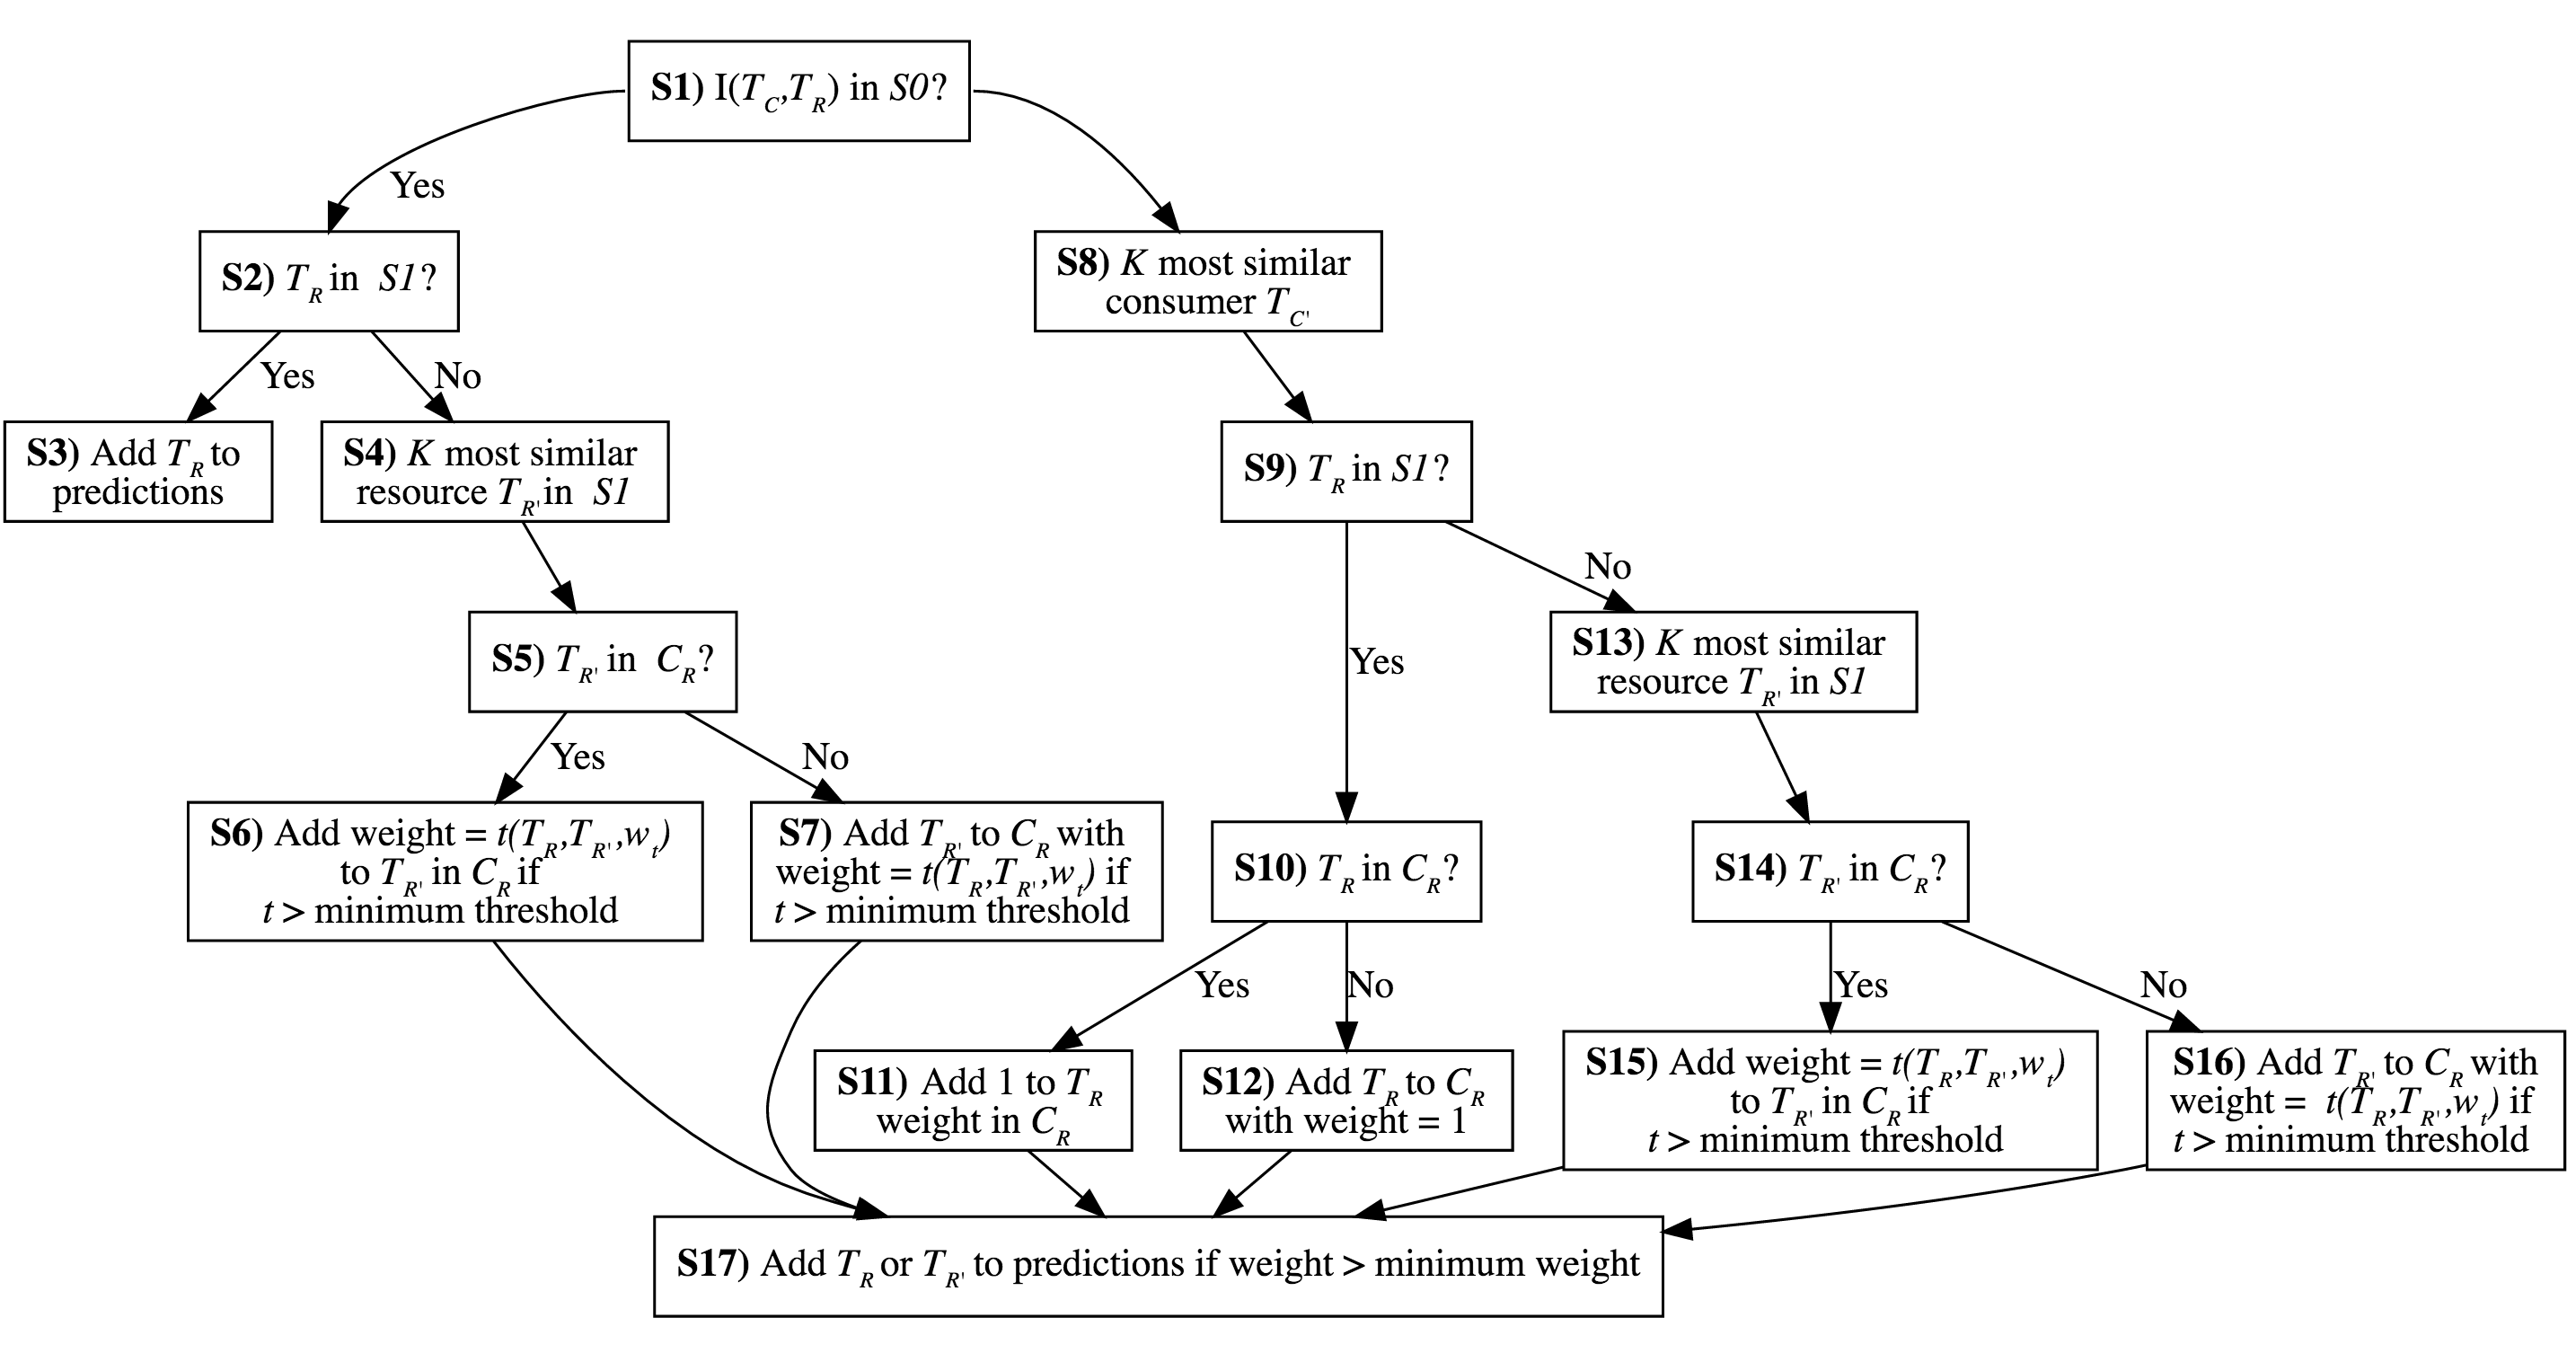
\includegraphics[width=\textwidth]{Decision_Diagram.png}
      \caption{Description of the logical steps used by the algorithm to suggest a list of candidate resources ($C_R$) for each consumer taxa ($T_C$) in an arbitrary set of $N_1$ for which interactions are predicted, using a set of taxa $N_0$ with empirically described interactions. Interactions between consumer and resource taxa are denoted as I($T_C$,$T_R$). $K$ is the number of most similar neighbours selected for the KNN algorithm, $t$ stands for tanimoto in equation 1, $w_t$ is the weight given to sets of resources and consumers in equation 2, the minimum threshold is an arbitrary value setting the minimal similarity value accepted for taxa to be considered as close neighbours in the KNN algorithm, the weight is the value added to a candidate resource each time it is added to $C_R$ and the minimum weight is the minimal weight value accepted for candidate resources to be selected as predicted sources in the algorithm.}
      \label{fig:decision_diag}
    \end{figure}

% Figure 2
\newpage
    \begin{figure}[h]
      \centering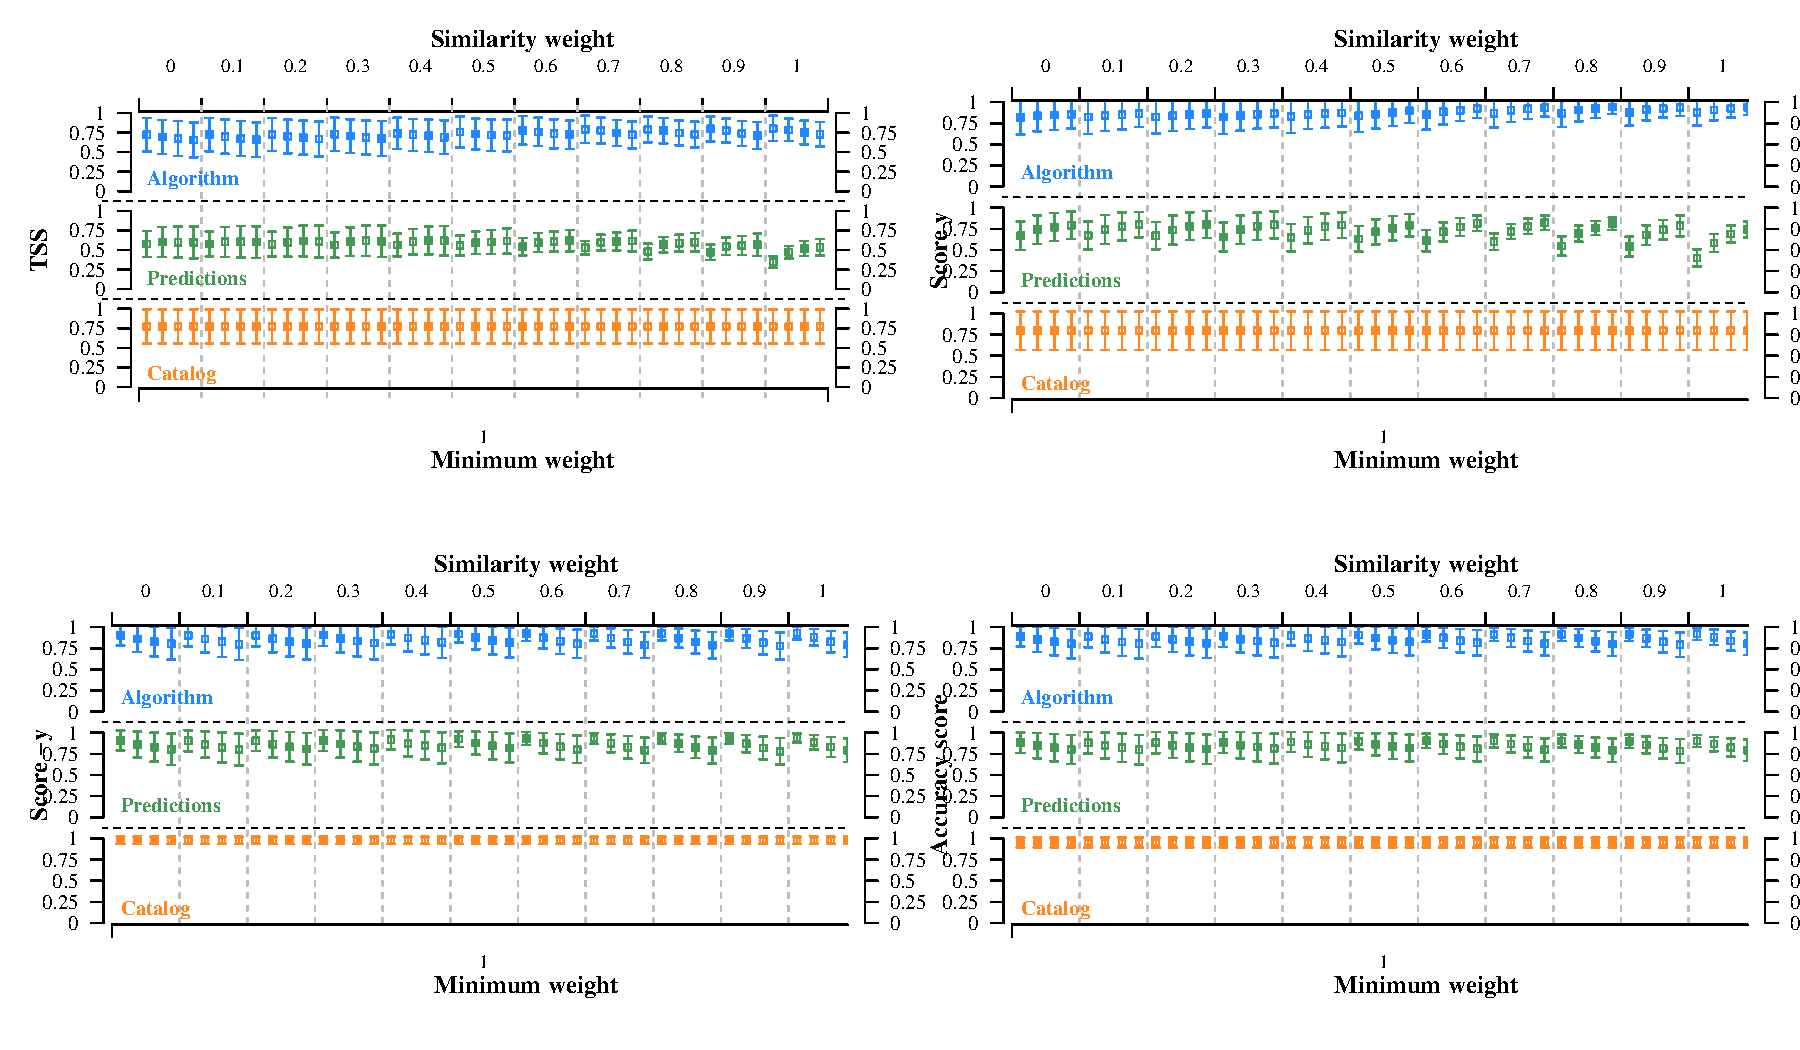
\includegraphics[width=\textwidth, height=12cm]{multiple_parameters2.pdf}
      \caption{The graph presents the three statistics as a function of trait weight, which varies between 0 and 1. A weight of 0 means that similarity is measured only using set of resources for each taxa, while a weight equal to 1 means that similarity is based solely on taxonomy. We present 6 food webs with over 50 taxa each and the Barnes et al. (2008) dataset.}
      \label{fig:multi_param}
    \end{figure}

% Figure 3
\newpage
    \begin{figure}[h]
      \centering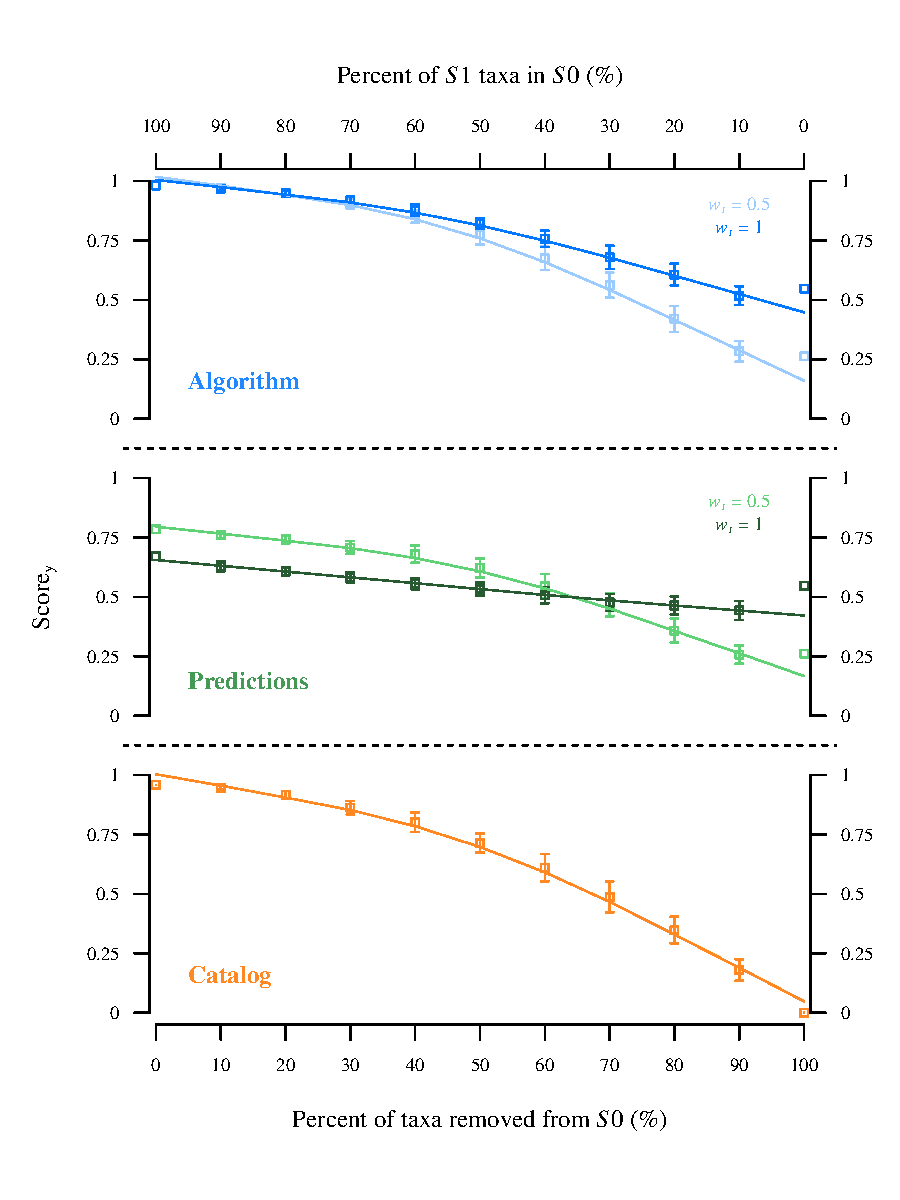
\includegraphics[width=\textwidth]{catalog_predictions2.pdf}
      \caption{Graph presenting predictive accuracy as a function of the amount of information available in the catalogue. The arctic food web from Kortsch et al. (2015) was used for this, as it is highly detailed and because almost all taxa found in it had information in the catalogue even when not included in the catalogue. A random percentage of taxa in the web was iteratively removed from the catalogue (n = 50) before predicting interactions with the XXX algorithm.}
      \label{fig:catalog_pred}
    \end{figure}

% Figure 4
\newpage
    \begin{figure}[h]
      \centering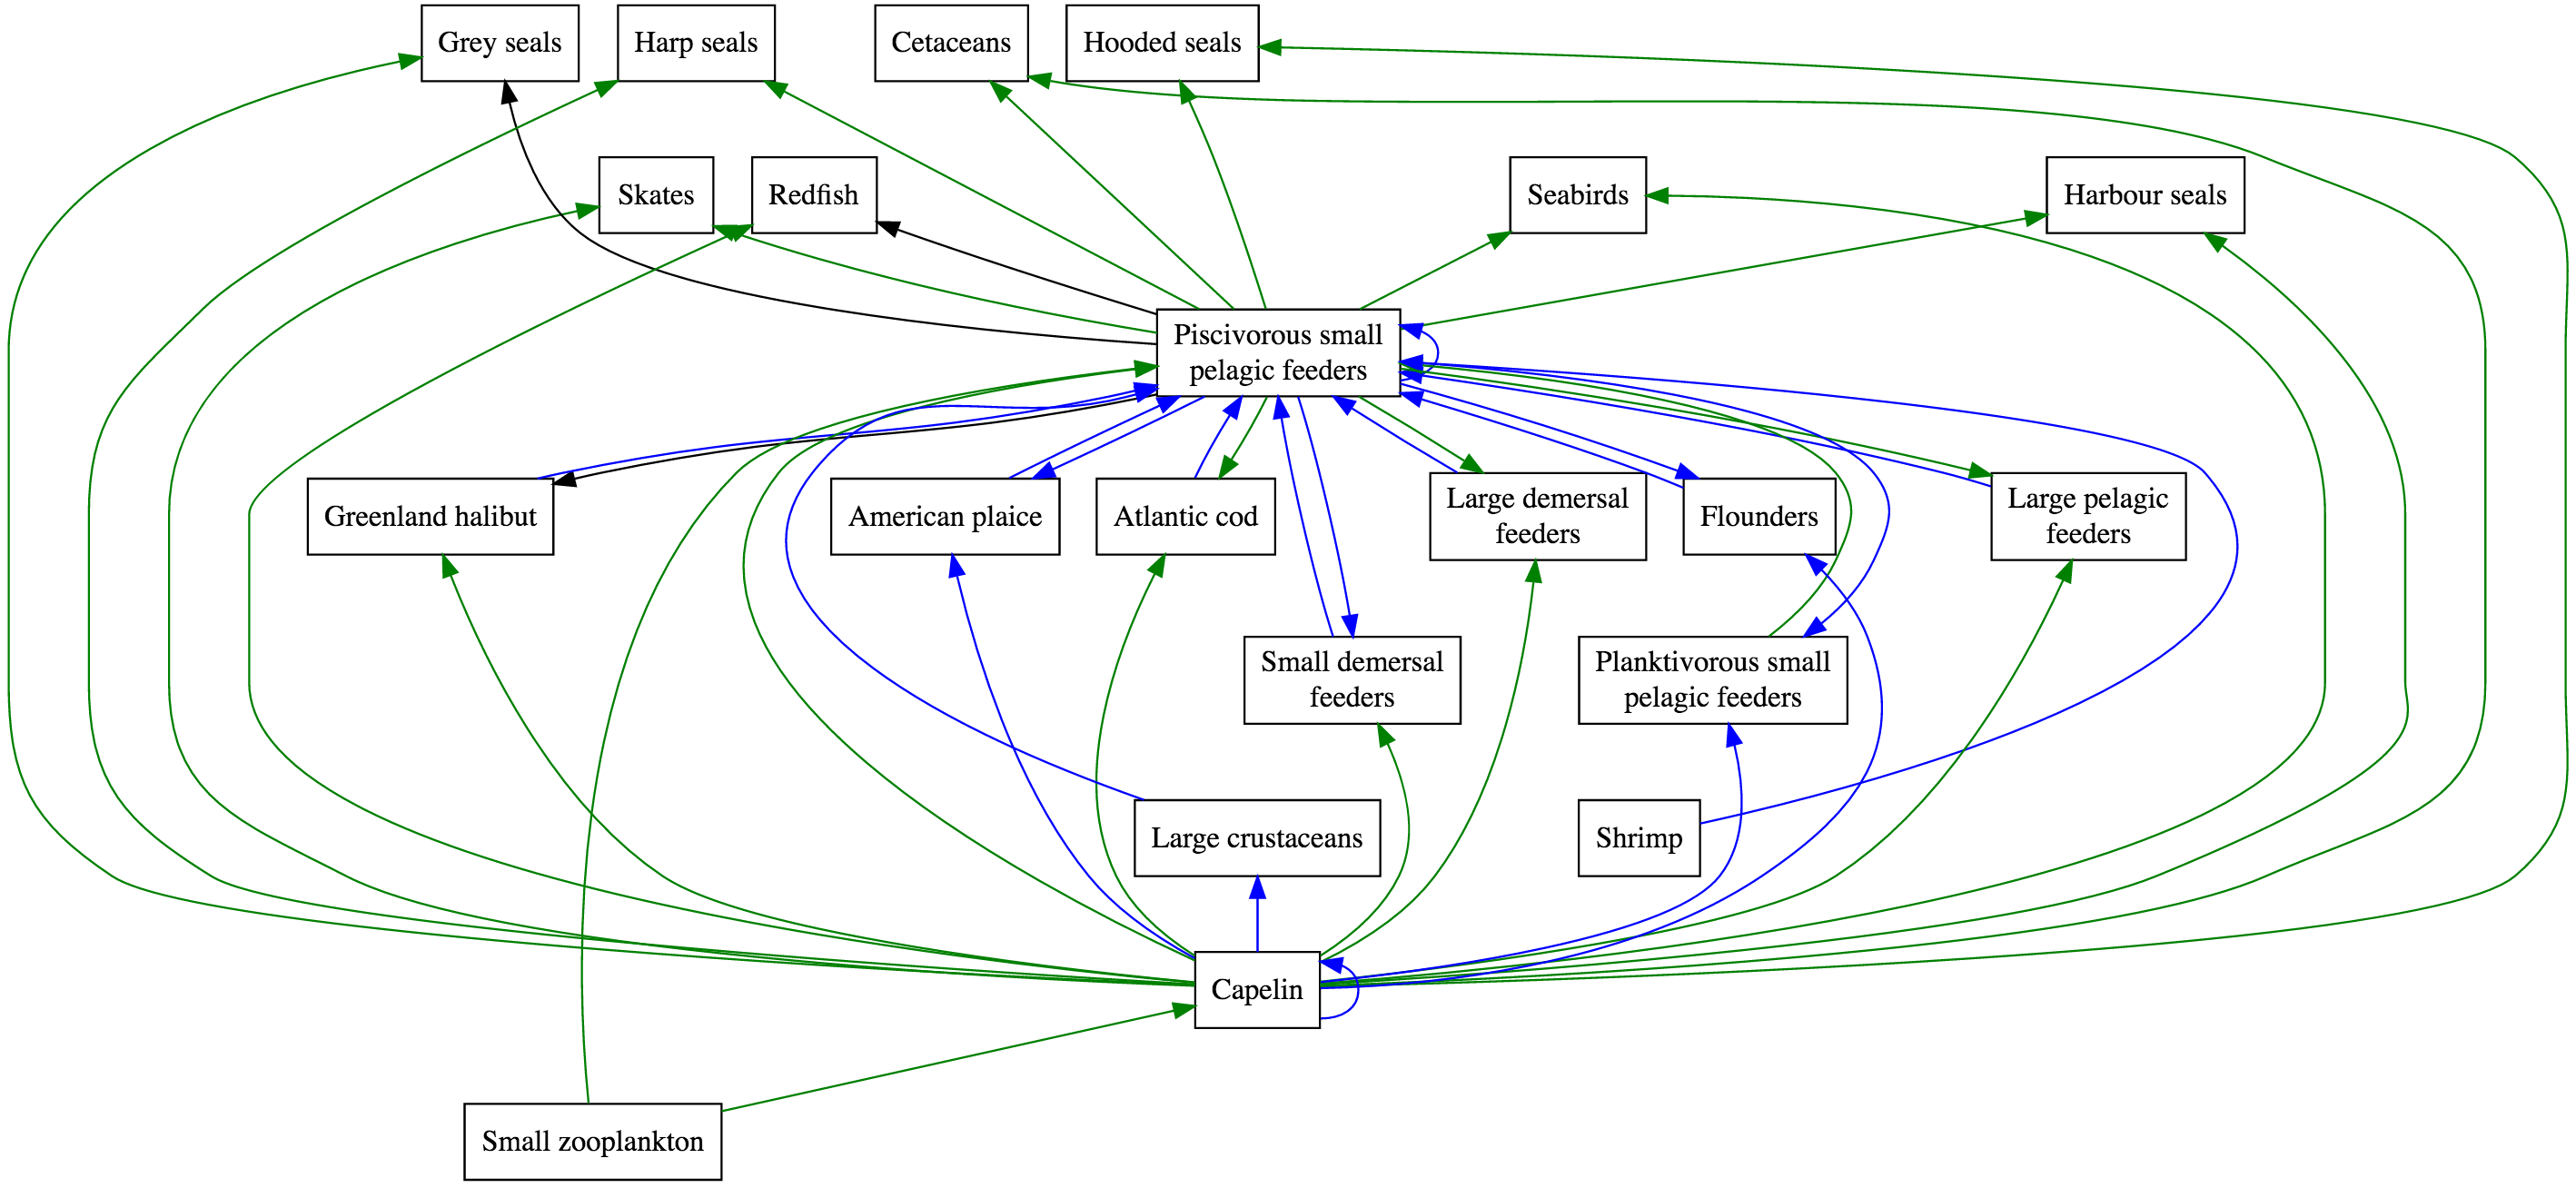
\includegraphics[width=\textwidth]{SGSL.png}
      \caption{Example of results from the algorithm with the Network of the Southern Gulf of Saint Lawrence (Savenkoff et al. 2004) centered on interactions of the capelin (\textit{Mallotus villosus}) and piscivorous small pelagic feeders (\textit{e.g. Scomber scombrus $and$ Illex illecebrosus}). Edge with colors green were both predicted and observed (26), black were observed only (3) and blue were predicted only (19).}
      \label{fig:SGSL}
    \end{figure}

\end{document}

% Cite taxize
% Scott Chamberlain and Eduard Szocs (2013). taxize - taxonomic search and retrieval in R. F1000Research, 2:191. URL: http://f1000research.com/articles/2-191/v2.
%
% Scott Chamberlain, Eduard Szocs, Carl Boettiger, Karthik Ram, Ignasi Bartomeus, and John Baumgartner (2014) taxize: Taxonomic information from around the web. R package version 0.3.0.
% https://github.com/ropensci/taxize
%
% Jorrit H. Poelen, James D. Simons and Chris J. Mungall. (2014). Global Biotic Interactions: An open infrastructure to share and analyze species-interaction datasets. Ecological Informatics. http://dx.doi.org/10.1016/j.ecoinf.2014.08.005
%
% Bailly, N.; Boury-Esnault, N.; Brandão, S.N.; Costello, M.J.; Gofas, S.; Hernandez, F.; Horton, T.; Kroh, A.; Mees, J.; Paulay, G.; Poore, G.; Rosenberg, G.; Stöhr, S.; Decock, W.; Dekeyzer, S.; Vandepitte, L.; Vanhoorne, B.; Vranken, S.; Adams, M.J.; Adlard, R.; Adriaens, P.; Agatha, S.; Ahn, K.J.; Ahyong, S.; Alvarez, B.; Anderson, G.; Angel, M.; Arango, C.; Artois, T.; Atkinson, S.; Barber, A.; Bartsch, I.; Bellan-Santini, D.; Berta, A.; Bieler, R.; Błażewicz-Paszkowycz, M.; Bock, P.; Böttger-Schnack, R.; Bouchet, P.; Boyko, C.B.; Bray, R.; Bruce, N.L.; Cairns, S.; Campinas Bezerra, T.N.; Cárdenas, P.; Carstens, E.; Catalano, S.; Cedhagen, T.; Chan, B.K.; Chan, T.Y.; Cheng, L.; Churchill, M.; Coleman, C.O.; Collins, A.G.; Crandall, K.A.; Cribb, T.; Dahdouh-Guebas, F.; Daly, M.; Daneliya, M.; Dauvin, J.C.; Davie, P.; De Grave, S.; de Mazancourt, V.; Defaye, D.; d'Hondt, J.L.; Dijkstra, H.; Dohrmann, M.; Dolan, J.; Drapun, I.; Eisendle-Flöckner, U.; Eitel, M.; Encarnação, S.C.d.; Epler, J.; Ewers-Saucedo, C.; Faber, M.; Feist, S.; Finn, J.; Fišer, C.; Fonseca, G.; Fordyce, E.; Foster, W.; Frank, J.H.; Fransen, C.; Furuya, H.; Galea, H.; Garcia-Alvarez, O.; Gasca, R.; Gaviria-Melo, S.; Gerken, S.; Gheerardyn, H.; Gibson, D.; Gil, J.; Gittenberger, A.; Glasby, C.; Glover, A.; Gordon, D.; Grabowski, M.; Gravili, C.; Guerra-García, J.M..; Guidetti, R.; Guilini, K.; Guiry, M.D.; Hajdu, E.; Hallermann, J.; Hayward, B.; Hendrycks, E.; Herrera Bachiller, A.; Ho, J.s.; Høeg, J.; Holovachov, O.; Hooper, J.; Hughes, L.; Hummon, W.; Hyzny, M.; Iseto, T.; Ivanenko, S.; Iwataki, M.; Jarms, G.; Jaume, D..; Jazdzewski, K.; Kaminski, M.; Karanovic, I.; Kim, Y.H.; King, R.; Kirk, P.M.; Kolb, J.; Kotov, A.; Krapp-Schickel, T.; Kremenetskaia, A.; Kristensen, R.; Kullander, S.; La Perna, R.; Lambert, G.; Lazarus, D.; LeCroy, S.; Leduc, D.; Lefkowitz, E.J.; Lemaitre, R.; Lörz, A.N.; Lowry, J.; Macpherson, E.; Madin, L.; Mah, C.; Mamos, T.; Manconi, R.; Mapstone, G.; Marshall, B.; Marshall, D.J.; McInnes, S.; Meidla, T.; Meland, K.; Merrin, K.; Messing, C.; Miljutin, D.; Mills, C.; Mokievsky, V.; Molodtsova, T.; Monniot, F.; Mooi, R.; Morandini, A.C.; Moreira da Rocha, R.; Moretzsohn, F.; Mortelmans, J.; Mortimer, J.; Musco, L.; Neubauer, T.A.; Neuhaus, B.; Ng, P.; Nielsen, C.; Nishikawa, T.; Norenburg, J.; O'Hara, T.; Okahashi, H.; Opresko, D.; Osawa, M.; Ota, Y.; Parker, A.; Patterson, D.; Paxton, H.; Perrier, V.; Perrin, W.; Petrescu, I.; Picton, B.; Pilger, J.F.; Pisera, A.; Polhemus, D.; Pugh, P.; Reimer, J.D.; Reuscher, M.; Rius, M.; Rützler, K.; Rzhavsky, A.; Saiz-Salinas, J.; Santos, S.; Sartori, A.F.; Satoh, A.; Schatz, H.; Schierwater, B.; Schmidt-Rhaesa, A.; Schneider, S.; Schönberg, C.; Schuchert, P.; Self-Sullivan, C.; Senna, A.R.; Serejo, C.; Shamsi, S.; Sharma, J.; Shenkar, N.; Sicinski, J.; Siegel, V.; Sinniger, F.; Sivell, D.; Sket, B.; Smit, H.; Smol, N.; Souza-Filho, J.F..; Stampar, S.N.; Sterrer, W.; Stienen, E.; Strand, M.; Suárez-Morales, E.; Summers, M.; Suttle, C.; Swalla, B.J.; Taiti, S.; Tandberg, A.H.; Tang, D.; Tasker, M.; Taylor, J.; Tchesunov, A.; ten Hove, H.; ter Poorten, J.J.; Thomas, J.; Thuesen, E.V.; Thurston, M.; Thuy, B.; Timi, J.T.; Timm, T.; Todaro, A.; Turon, X.; Tyler, S.; Uetz, P.; Utevsky, S.; Vacelet, J.; Vader, W.; Väinölä, R.; van der Meij, S.E.; van Ofwegen, L.; van Soest, R.; Van Syoc, R.; Venekey, V.; Vonk, R.; Vos, C.; Walker-Smith, G.; Walter, T.C.; Watling, L.; Whipps, C.; White, K.; Williams, G.; Wilson, R.; Wyatt, N.; Wylezich, C.; Yasuhara, M.; Zanol, J.; Zeidler, W. (2016). World Register of Marine Species. Available from http://www.marinespecies.org at VLIZ. Accessed 2016-09-13. doi:10.14284/170
